\documentclass[10pt,journal,twocolumn]{IEEEtran}
\usepackage[T1]{fontenc}
\usepackage{amsmath,amssymb,graphicx,booktabs,url}
\usepackage[hidelinks]{hyperref}
\hypersetup{pdftitle={Neighbor Work Sharing on Master-Centered Platonic-Solid Networks},pdfauthor={Study manuscript},pdfsubject={Reproducible discrete-event simulation study},pdfkeywords={Platonic solids, work sharing, scheduling, simulation}}
\graphicspath{{figures/}}
\newcommand{\push}{neighbor push}
\title{Neighbor Work Sharing on Master-Centered Platonic-Solid Networks: A Reproducible Simulation Study}
\author{Study manuscript\thanks{Author names and affiliations are left for the study owner to supply. All reported performance measurements are discrete-event simulation results. This manuscript has not been submitted to or endorsed by IEEE.}}
\markboth{Reproducible Simulation Study}{Neighbor Work Sharing on Platonic-Solid Networks}
\begin{document}
\maketitle

\begin{abstract}
We study a homogeneous master--worker system in which workers occupy the vertices of a Platonic solid, each worker has a direct link to the central master, and peer links follow the solid's edges. The master simultaneously dispatches equal-count task chunks. Busy workers subsequently donate queued independent tasks to idle adjacent workers, and every completed task returns its identified result to the master. A discrete-event simulator includes fixed link bandwidth and latency, link serialization, explicit idle notifications, reservation handshakes, nonpreemptive execution, and result collection. We compare this policy with six scheduling alternatives on all five Platonic solids, using identical task instances and physical networks within each comparison. Five workload families, communication sensitivities, and five alternative peer topologies yield 16,050 simulation runs. At 100 MiB/s and 10 microseconds one-way latency, neighbor sharing provides mean paired speedups of 1.074--1.228 over static partitioning for independent lognormal task costs and 2.763--5.630 for an intentionally clustered stress workload. It provides no speedup for equal-cost tasks and has the lowest mean makespan in only one of twenty variable-cost scheduler comparisons. Degree-matched topology controls do not establish a general advantage of Platonic connectivity. The evidence supports neighbor sharing as a useful load-balancing policy, while qualifying claims of geometric or scheduler superiority.
\end{abstract}

\begin{IEEEkeywords}
Distributed scheduling, load balancing, work sharing, work stealing, Platonic solids, discrete-event simulation.
\end{IEEEkeywords}

\section{Introduction}
\IEEEPARstart{A}{n} equal division of task counts is not necessarily an equal division of computation. Even with identical processors and stable communication links, independent tasks of different costs can leave some workers idle while others retain substantial queued work. The system studied here uses a central master and a regular geometric peer graph to redistribute that remaining work locally.

The master occupies the center of a tetrahedron, cube, octahedron, dodecahedron, or icosahedron. Workers occupy its vertices. A worker communicates directly with the master and with workers joined to it by solid edges. After receiving an equal-count initial chunk, it executes tasks sequentially. When an adjacent worker is idle, a busy worker can transfer queued tasks to it. Tasks retain their original identifiers throughout redistribution; their results are returned directly to the master as they finish.

Three questions guide the study: (1) how much does neighbor sharing improve on static equal partitioning; (2) how does it compare with reasonable centralized and distributed scheduling alternatives; and (3) do results support an advantage specific to Platonic peer connectivity? The third question requires topology controls. Strong scaling from four to twenty workers alone cannot demonstrate a geometric advantage.

We contribute a reproducible event model, a task-ownership protocol, paired measurements with uncertainty estimates, and communication and topology ablations. Results are reported whether or not they favor the proposed policy. These are synthetic simulation measurements, not observations from a physical cluster or comparisons with deployed software products.

\section{Related Scheduling Approaches}
Adaptive load sharing in homogeneous distributed systems predates this study; Eager, Lazowska, and Zahorjan examine that setting~\cite{eager}. Work stealing provides a receiver-initiated alternative. Blumofe and Leiserson analyze randomized stealing for multithreaded computations~\cite{blumofe}; their theoretical guarantees concern a different computation and runtime model and are not assumed to apply to the finite networks here.

Central self-scheduling assigns work when a worker asks for it. Guided self-scheduling decreases batch sizes as work runs out~\cite{guided}. Our guided comparator uses a documented configurable variant with divisor $2N$. Classical scheduling bounds motivate the compute-only lower bound used below~\cite{graham}. The regular-solid construction follows standard Platonic geometry~\cite{coxeter}.

The contribution is the controlled evaluation of this particular master-centered, edge-restricted protocol. We do not claim that work donation, work stealing, or Platonic graphs are newly invented. The comparators are explicit abstract scheduling policies inspired by the literature, rather than complete implementations of named distributed-computing frameworks.

\section{System and Communication Model}
\subsection{Geometry and Hardware Assumptions}
Let $G=(V,E)$ be the undirected worker graph and $N=|V|$. A master $m$ adds spokes $(m,v)$ for every $v\in V$. Table~\ref{tab:geometry} gives the physical peer graphs. The dodecahedron has twenty workers of peer degree three; the icosahedron has twelve workers of peer degree five. They have the same thirty peer edges but different processor counts. Including the master, there are $N+1$ homogeneous nodes.

\begin{table}[!t]
\caption{Platonic worker graphs; master spokes are additional.}
\label{tab:geometry}\centering
\begin{tabular}{lrrrr}
\toprule Solid & Workers & Peer edges & Peer degree & Faces \\
\midrule
Tetrahedron & 4 & 6 & 3 & 4 \\
Cube & 8 & 12 & 3 & 6 \\
Octahedron & 6 & 12 & 4 & 8 \\
Dodecahedron & 20 & 30 & 3 & 12 \\
Icosahedron & 12 & 30 & 5 & 20 \\
\bottomrule
\end{tabular}
\end{table}

\begin{figure*}[!t]
\centering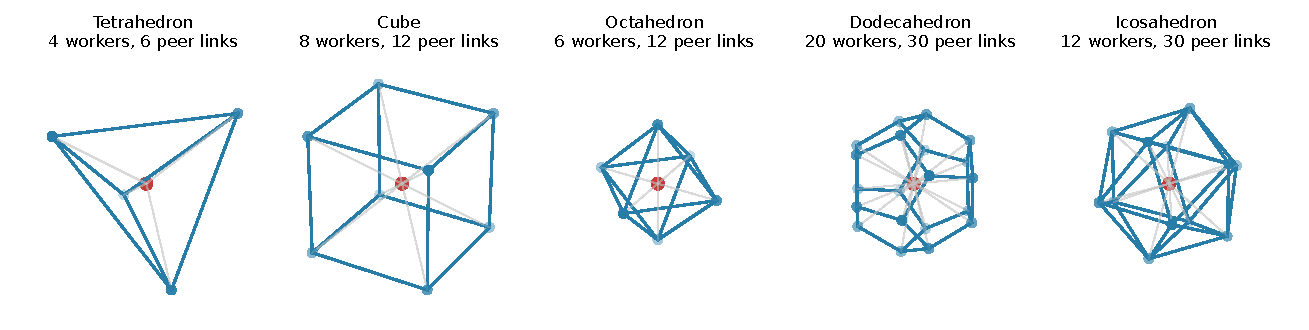
\includegraphics[width=\textwidth]{solids.pdf}
\caption{Actual solid vertex coordinates and shortest-distance edges. Blue points are workers, blue lines are peer links, the red point is the master, and gray lines are master spokes. Geometry specifies adjacency; link speed and propagation latency are identical regardless of physical length.}
\label{fig:solids}
\end{figure*}

Each worker has one identical processing lane. The master performs scheduling and result collection; it does not execute application tasks. Its hardware is not assumed faster than the workers'. Application computation and communication can overlap. The primary model assigns zero CPU cost to scheduling and message handling at all nodes; a separate sensitivity adds a serialized processing requirement at the master. No failures, fluctuating capacities, task dependencies, replication, or task cancellation are modeled.

All physical links have fixed one-way propagation latency $L$ and bandwidth $B$. In the primary model, each direction of each link has its own serializer; opposite directions are full duplex and different links operate concurrently. For a message of $b$ bytes sent at time $t$, its serialization starts at
\begin{equation}
t_s=\max(t,A_{uv}),\quad t_a=t_s+b/B+L,
\end{equation}
where $A_{uv}$ is the next free serialization time of directed link $(u,v)$. After dispatch, $A_{uv}$ becomes $t_s+b/B$. Propagation does not hold the serializer. Control messages, task batches, and results use the same FIFO link resources. Waiting time can vary because of queues; bandwidth and propagation speed remain constant.

A message between nonadjacent workers is routed through the master with store-and-forward serialization and propagation on both physical hops. No comparator receives an unmodeled direct worker link. Global stealing uses direct peer edges where available and the two-hop master route otherwise.

The primary experiment has $L=0.01$ ms (10 $\mu$s), $B=100$ MiB/s, a 4,096-byte input per task, 64-byte results, and 32-byte message headers or control packets. A batch containing $k$ tasks occupies $32+4096k$ bytes. Task and result sizes include their identifiers. Sizes are fixed; computation costs vary independently of size. Link parameters are explicit assumptions rather than measured hardware characteristics.

\subsection{Tasks, Initialization, and Completion}
There are $M=2400$ independent tasks with unique IDs $0,\ldots,M-1$. All five worker counts divide $M$. A cost $c_i>0$ is the time needed by any worker to execute task $i$. Schedulers cannot inspect these costs. Costs are normalized per instance so $\sum_i c_i=2400$ ms; the mean task therefore takes 1 ms. The same IDs, sizes, order, and costs are reused across policies and solids for a workload seed.

Equal-initial-partition policies divide the ordered IDs into $N$ contiguous chunks of $M/N$ tasks. Chunk-to-vertex mapping is randomly permuted for each seed, preventing a fixed association between task cost and coordinate labels. At time zero, the master initiates one transfer on every spoke. In the independent-link model, transfers serialize concurrently and arrive simultaneously. The shared-NIC sensitivity necessarily constrains this physical concurrency.

A worker executes one task at a time, nonpreemptively, and immediately sends each completed result to the master. Running tasks cannot move. Only not-yet-started IDs can be donated. A recipient can later donate received queued tasks to its own neighbors. Results retain the original ID and go directly to the master, including for tasks that migrated multiple times.

Makespan $T$ ends when the master receives the last result, rather than when the last worker finishes computation. A compute-only lower bound and utilization are
\begin{equation}
T_{\rm LB}=\max\left(\frac{\sum_i c_i}{N},\max_i c_i\right),\qquad
U=\frac{\sum_i c_i}{NT}.
\end{equation}
This bound excludes distribution and collection costs and need not be achievable. Master utilization is excluded because it does not process application tasks.

\section{Policies and Task Ownership}
\subsection{Neighbor Push Protocol}
The proposed policy uses messages rather than instantaneous global knowledge. An idle worker announces an \texttt{IDLE} epoch to adjacent workers. Becoming active sends a corresponding \texttt{BUSY} notice. A busy donor with queued work and a recorded idle neighbor reserves a fraction $f=1/2$ of its currently unreserved queue, rounded up, and sends an \texttt{OFFER}. The donor continues executing its running task; reserved tasks await the receiver's decision.

The receiver accepts the first offer only if it remains idle, its idle epoch matches, and no earlier accepted transfer is outstanding. It rejects competing or stale offers. Upon \texttt{ACCEPT}, the donor transfers the reserved IDs and inputs over the direct edge. Upon \texttt{REJECT}, it restores those IDs to its queue. Each message has the modeled delay and byte cost. The handshake prevents double assignment to an idle recipient and removes reliance on perfect instantaneous knowledge. Neighbors are considered in seeded random order. There is no batch cap in the primary policy.

An ID has exactly one logical owner: the master pool, a worker queue, a running worker, an offer reservation, a data transfer, or the completed set. Starting an ID twice, completing it twice, or collecting its result twice triggers an assertion. Small validation runs additionally inspect ownership after every event. Exactly-once execution in this failure-free model does not imply fault-tolerant exactly-once behavior after crashes.

\subsection{Six Competitors}
All competitors use the same $N$ workers and available links:
\begin{enumerate}
\item \emph{Static}: equal initial chunks, without redistribution.
\item \emph{Neighbor steal}: an idle worker requests work from a random untried adjacent worker. A donor immediately removes and transfers half its queued tasks, or returns an empty reply.
\item \emph{Global steal}: the same half-queue policy, with donors sampled from all other workers. Nonadjacent requests, replies, and data traverse the master.
\item \emph{Master rebalance}: after equal initial chunks, an idle worker asks the master. The master probes donors in random order until one returns queued work, then forwards the donated half-queue batch to the idle worker. The master has no oracle for actual remaining costs or instantaneous queues.
\item \emph{Master queue (1)}: tasks initially remain at the master. Idle workers request one task at a time.
\item \emph{Guided queue}: tasks initially remain at the master. A request receives $\max(1,\lceil R/(2N)\rceil)$ tasks, where $R$ is the remaining pool count.
\end{enumerate}

Queue-based competitors intentionally change initial allocation as part of their scheduling design. They have the same total work and communication resources and pay all request and transfer costs. The other five policies share equal-count initialization. Half-queue donation affects neighbor/global stealing and master rebalancing equally. Empty stealing sweeps and unsuccessful master rebalance sweeps wait 1 ms before retrying; otherwise, a thief does not stop permanently while work may reappear. Definitive empty master pools stop issuing work. Completion ends the simulation before unneeded retry events are drained.

\section{Experiment Design and Validation}
\subsection{Workloads and Paired Repetition}
Five workload families are evaluated:
\begin{itemize}
\item \emph{Constant}: every task costs 1 ms. This checks that identical compute and equal chunks provide no redistribution opportunity.
\item \emph{Exponential}: independent unit-mean exponential costs before per-instance normalization.
\item \emph{Lognormal}: independent costs with pre-normalization population coefficient of variation two, using $\sigma^2=\ln 5$ and log-mean $-\sigma^2/2$.
\item \emph{Pareto}: $\min(1+X,100)$, where $X$ is a Lomax draw with shape 1.5, followed by normalization. This is a capped heavy-tail workload, not an unbounded infinite-variance workload.
\item \emph{Clustered}: the same lognormal draws sorted by cost before equal chunks are formed. This deliberately concentrates expensive tasks in a few chunks. Chunk locations are then permuted among vertices.
\end{itemize}

The clustered case is an artificial stress scenario for correlated chunk costs, not a typical measured application. It also preserves ascending task order in the master pool, so queue policies must cope with expensive tasks appearing late. The independent lognormal workload is the more neutral heterogeneity comparison. Normalization gives identical total computation to all instances while retaining task-cost imbalance.

Each primary cell uses thirty workload seeds $0$--$29$. Scheduler seed is workload seed plus 70,001. Policies share initial chunk placement; their later random choices can diverge as their event histories diverge. There are $5\times5\times30\times7=5250$ primary runs. Four processes run independent cases; this execution parallelism does not enter simulated timing.

For each seed, speedup relative to static is $T_{\rm static}/T_{\rm policy}$. Reported speedups are means of these paired ratios, not ratios of reported means. Uncertainty intervals use 10,000 percentile bootstrap resamples of paired seed observations with fixed analysis seed 192,024. Mean makespan intervals bootstrap the observed makespans. Constant workloads have deterministic timing in the primary model. Intervals are exploratory, cell-wise 95\% intervals without multiple-comparison correction; lowest means alone do not establish statistical superiority.

\subsection{Sensitivity and Topology Controls}
Communication and policy sensitivity uses the icosahedron and dodecahedron, lognormal and clustered work, and fifteen seeds per setting. It varies latency (1, 100, and 1000 $\mu$s in addition to the 10-$\mu$s baseline), bandwidth (10 and 1000 MiB/s in addition to 100), a shared NIC, a 10-$\mu$s master service cost per incoming physical-hop message, their combination, donation fractions 1/4 and 3/4, an eight-task donation cap, retry intervals 0.1 and 10 ms, and task counts 120 and 9600. There are 6300 sensitivity runs. Figures compare the baseline's first fifteen seeds with these same fifteen seeds, avoiding an unpaired thirty-versus-fifteen comparison.

The shared-NIC model adds one transmit and one receive serializer per node, both at $B$. A transfer waits for its link and both endpoint resources; FIFO reservations can create head-of-line blocking. Opposite directions remain independent. It is a specific resource-contention sensitivity, not a model of every network switch. The master service sensitivity introduces a scheduling/collection processing workload on the otherwise identical master; worker control costs remain zero.

Five peer-topology alternatives retain the same master and $N$ workers: no peer edges (a master star), a worker ring, a rectangular nearest-neighbor grid, a connected degree-preserving rewiring of the Platonic graph, and complete peer connectivity. Grid dimensions are $2\times2$, $2\times4$, $2\times3$, $4\times5$, and $3\times4$ for the five solid sizes. Neighbor push and neighbor steal are tested on each alternative with thirty seeds for lognormal, Pareto, and clustered work, adding 4500 runs. Complete graphs and rings change link counts, so they are capacity and sparsity references, not equal-cost hardware comparisons. Rewired controls preserve peer degree and peer edge count.

The rewiring uses 100 attempted double-edge swaps per original edge and rejects disconnected outcomes. Its graph seed is workload seed plus 90,001. It is not claimed to sample regular graphs uniformly. Tetrahedral degree-three connectivity on four vertices is already complete; the octahedral four-regular graph on six vertices is unique up to relabeling. Those controls cannot identify a distinct topological advantage. Randomized graph labels can still change finite-seed paired outcomes.

\subsection{Readiness and Correctness Checks}
The validation suite has 116 passing tests. Geometry checks verify vertex and edge counts, regular degree, connectedness, circumradius, Euler's relation, and the number of unique convex-hull supporting planes. Edge construction uses the minimum positive Euclidean vertex distance, rather than arbitrary near-neighbor wiring.

An analytic static check computes the equal-spoke input-transfer time plus the largest chunk cost plus one result-transfer time. Other tests verify every policy and solid with shared-NIC and master-service variants, ownership at every event, nonadjacent routing, zero-overhead equal-cost completion, redistribution of a known imbalance, inability to migrate a running long task, and slow-link reservation races. Alternative peer graphs are also checked. Every measured run asserts that all $M$ IDs executed once and all $M$ results reached the master, and that $T\geq T_{\rm LB}$. Passing these checks establishes internal model consistency, not empirical validation against physical hardware.

\section{Results}
\subsection{Makespan Across All Five Solids}
Table~\ref{tab:results} reports every primary workload--solid cell for all seven policies. Table~\ref{tab:speed} gives selected paired speedups and confidence intervals. Figure~\ref{fig:effects} summarizes comparisons with static and neighbor stealing.

\begin{table*}[!t]
\caption{Mean last-result makespan (ms), thirty paired seeds per cell, 2400 tasks. Bold denotes the smallest observed mean, not a significance claim. Solids have different worker counts; policy comparisons within a row have identical hardware and task instances.}
\label{tab:results}\centering\scriptsize
\begin{tabular}{llrrrrrrr}
\toprule
Workload & Solid & Static & Push & N. steal & G. steal & Rebalance & Queue (1) & Guided \\
\midrule
Constant & Tetra. & 623.46 & 623.46 & 623.46 & 623.46 & 623.46 & 636.18 & 623.70 \\
Constant & Cube & 311.74 & 311.74 & 311.74 & 311.74 & 311.74 & 318.09 & 311.96 \\
Constant & Octa. & 415.65 & 415.65 & 415.65 & 415.65 & 415.65 & 424.12 & 415.89 \\
Constant & Dodeca. & 124.71 & 124.71 & 124.71 & 124.71 & 124.71 & 127.24 & 124.91 \\
Constant & Icosa. & 207.83 & 207.83 & 207.83 & 207.83 & 207.83 & 212.07 & 208.06 \\
\midrule
Exponential & Tetra. & 647.91 & 625.35 & 625.38 & 625.38 & 625.90 & 637.39 & 624.89 \\
Exponential & Cube & 340.11 & 314.73 & 314.07 & 314.72 & 314.68 & 319.92 & 313.86 \\
Exponential & Octa. & 443.85 & 417.90 & 417.98 & 417.86 & 418.20 & 425.72 & 417.61 \\
Exponential & Dodeca. & 146.47 & 128.83 & 128.67 & 128.47 & 128.30 & 129.97 & 127.72 \\
Exponential & Icosa. & 232.46 & 210.46 & 210.38 & 210.73 & 211.04 & 214.26 & 210.34 \\
\midrule
Lognormal & Tetra. & 673.96 & 627.77 & 627.41 & 627.41 & 628.65 & 639.84 & 627.63 \\
Lognormal & Cube & 362.04 & 318.24 & 317.41 & 318.77 & 318.78 & 324.06 & 319.47 \\
Lognormal & Octa. & 466.45 & 422.65 & 422.07 & 422.21 & 423.36 & 429.19 & 422.03 \\
Lognormal & Dodeca. & 169.65 & 138.73 & 138.83 & 138.78 & 138.41 & 138.59 & 137.53 \\
Lognormal & Icosa. & 255.70 & 216.23 & 216.05 & 216.08 & 216.73 & 219.90 & 217.79 \\
\midrule
Pareto & Tetra. & 675.19 & 630.17 & 629.28 & 629.28 & 631.74 & 640.01 & 628.86 \\
Pareto & Cube & 363.55 & 322.13 & 321.09 & 321.64 & 321.41 & 326.18 & 322.62 \\
Pareto & Octa. & 467.89 & 423.65 & 421.92 & 422.13 & 424.50 & 430.26 & 423.95 \\
Pareto & Dodeca. & 174.38 & 143.05 & 141.58 & 142.19 & 142.49 & 142.44 & 141.61 \\
Pareto & Icosa. & 259.67 & 220.76 & 219.80 & 220.50 & 221.51 & 223.24 & 221.30 \\
\midrule
Clustered & Tetra. & 1751.72 & 634.05 & 633.87 & 633.87 & 641.48 & 654.99 & 642.56 \\
Clustered & Cube & 1312.11 & 323.32 & 322.82 & 322.66 & 325.59 & 341.79 & 335.81 \\
Clustered & Octa. & 1488.81 & 424.99 & 425.03 & 425.87 & 431.02 & 446.23 & 438.84 \\
Clustered & Dodeca. & 834.65 & 148.54 & 150.37 & 137.60 & 137.27 & 154.84 & 152.99 \\
Clustered & Icosa. & 1083.71 & 220.39 & 219.03 & 218.30 & 220.39 & 237.81 & 234.28 \\
\midrule
\bottomrule
\end{tabular}

\end{table*}

\begin{table*}[!t]
\caption{Neighbor-push speedup over static: mean paired ratio and exploratory 95\% bootstrap interval. Total task count and total computation are identical across solids; worker count differs.}
\label{tab:speed}\centering
\begin{tabular}{lrr}
\toprule
Solid & IID lognormal & Clustered \\
\midrule
Tetra. & 1.074 [1.061, 1.087] & 2.763 [2.750, 2.775] \\
Cube & 1.137 [1.119, 1.157] & 4.059 [4.017, 4.100] \\
Octa. & 1.104 [1.085, 1.124] & 3.503 [3.480, 3.527] \\
Dodeca. & 1.228 [1.184, 1.274] & 5.630 [5.522, 5.730] \\
Icosa. & 1.183 [1.156, 1.211] & 4.923 [4.850, 4.997] \\
\bottomrule
\end{tabular}

\end{table*}

\begin{figure*}[!t]
\centering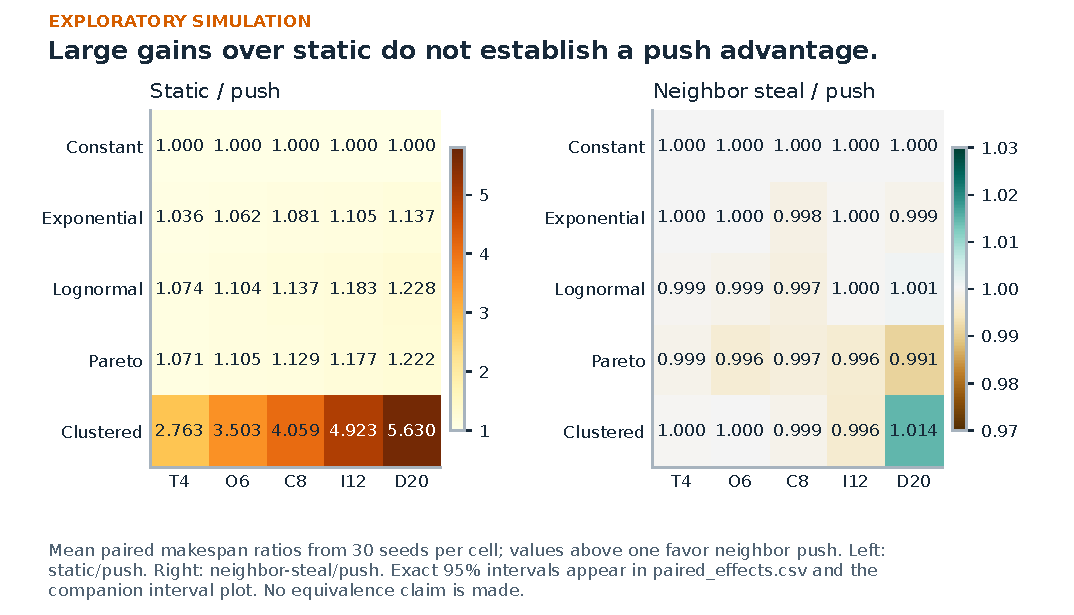
\includegraphics[width=.90\textwidth]{paired_effects.pdf}
\caption{Mean paired makespan ratios. A value above one favors neighbor push. Large improvements over static do not translate into consistent improvements over neighbor stealing. Exact intervals are in the accompanying paired-effects CSV; clustered neighbor-steal intervals all include one.}
\label{fig:effects}
\end{figure*}

Equal-cost results are identical across static and equal-initial-chunk redistribution policies. For $N$ workers, the common primary makespan is
\begin{equation}
T=\frac{2400}{N}+2L+\frac{32+4096(2400/N)+64}{B}.
\end{equation}
For example, this is 207.83 ms for the icosahedron and 124.71 ms for the dodecahedron. All workers finish their equally costly chunks together, so there is no useful idle neighbor before completion. A master queue adds per-request latency or additional batch boundaries; it cannot be expected to improve this balanced case.

For independent lognormal costs, mean push makespan is 216.23 ms on the icosahedron and 138.73 ms on the dodecahedron. Their static means are 255.70 and 169.65 ms. Mean paired speedups are 1.183 and 1.228. Across all solids, independent lognormal speedups range from 1.074 to 1.228. Exponential and capped-Pareto workloads also improve over static, but the exact effect depends on task variability, worker count, and the longest indivisible task.

The clustered stress workload shows much larger improvements: icosahedral makespan falls from 1083.71 to 220.39 ms; dodecahedral makespan falls from 834.65 to 148.54 ms. Mean paired speedups are 4.923 [4.850, 4.997] and 5.630 [5.522, 5.730], respectively. These gains reflect severe initial imbalance and available queued work. They should not be generalized to well-mixed or equal-cost tasks.

\subsection{Competitive Scheduling Performance}
Neighbor push has the lowest observed mean in one of twenty variable-cost primary cells: the octahedral clustered workload. Even there, its 424.99-ms mean is nearly equal to neighbor stealing's 425.03 ms. In the clustered workload, the neighbor-steal/push paired confidence interval contains one for every solid. Thus those observations do not establish a consistent push advantage over local stealing.

On the dodecahedron's clustered workload, master rebalancing has a 137.27-ms mean and global stealing 137.60 ms, compared with 148.54 ms for push and 150.37 ms for neighbor stealing. The dodecahedron has only three peers per worker, so locality restricts which idle workers can help a busy chunk. Global access can use idle capacity beyond that immediate neighborhood, at the cost of more master traffic. Guided scheduling has the best mean on several independent-cost cells; the icosahedral lognormal mean is 217.79 ms, slightly above local stealing's 216.05 ms and push's 216.23 ms.

The result is a useful but qualified finding: neighbor sharing addresses imbalance relative to static allocation, while established policy alternatives often match it or perform better. Lowest-mean counts are descriptive and depend on the specified synthetic workloads and parameters.

\subsection{Communication and Master Traffic}
\begin{figure*}[!t]
\centering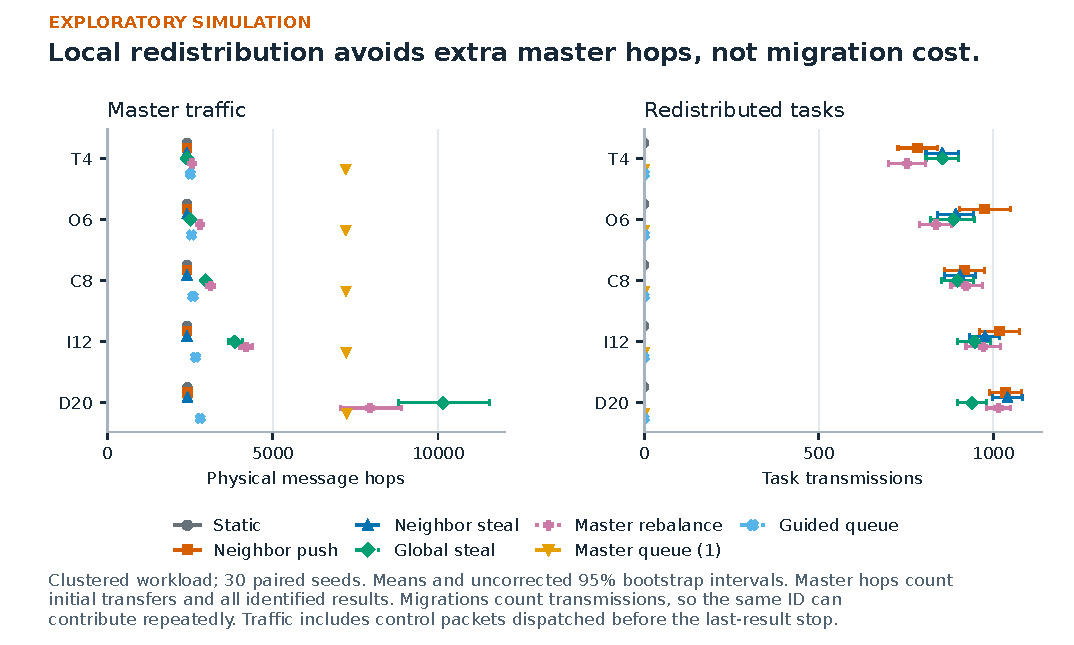
\includegraphics[width=.90\textwidth]{traffic.pdf}
\caption{Clustered-workload traffic, thirty seeds. Master hops include the initial distribution and all per-task results. Migration counts count task transmissions, so an ID can contribute more than once. Traffic records messages dispatched before the last-result stopping time, including outstanding control messages.}
\label{fig:traffic}
\end{figure*}

Local push and local stealing generate the same baseline master-hop count as static: $M+N$, or 2412 on the icosahedron and 2420 on the dodecahedron. Their redistribution control and data stay on peer edges. Every result still visits the master, so this avoids additional redistribution traffic rather than removing the master from the system.

For clustered dodecahedral work, push dispatches a mean 3934.53 physical-hop messages in total, with 2420 master hops; master rebalancing dispatches 7941.60 master hops. Single-task central scheduling dispatches 7239 master hops. Guided batching needs only 2809. Thus a centralized policy can also keep scheduling traffic modest through batching.

On the same dodecahedral workload, push migrates a mean 1035.40 task transmissions and dispatches 14.27 MB of physical-hop traffic (decimal bytes). Static dispatches 9.98 MB. Rebalancing dispatches 18.48 MB because donated data travels through the master. These are total sent bytes, not payload copied only once; forwarding and repeat migration are counted. Lower master traffic does not automatically imply the lowest makespan under independent links and zero scheduling CPU cost.

\subsection{Communication Sensitivity}
\begin{figure*}[!t]
\centering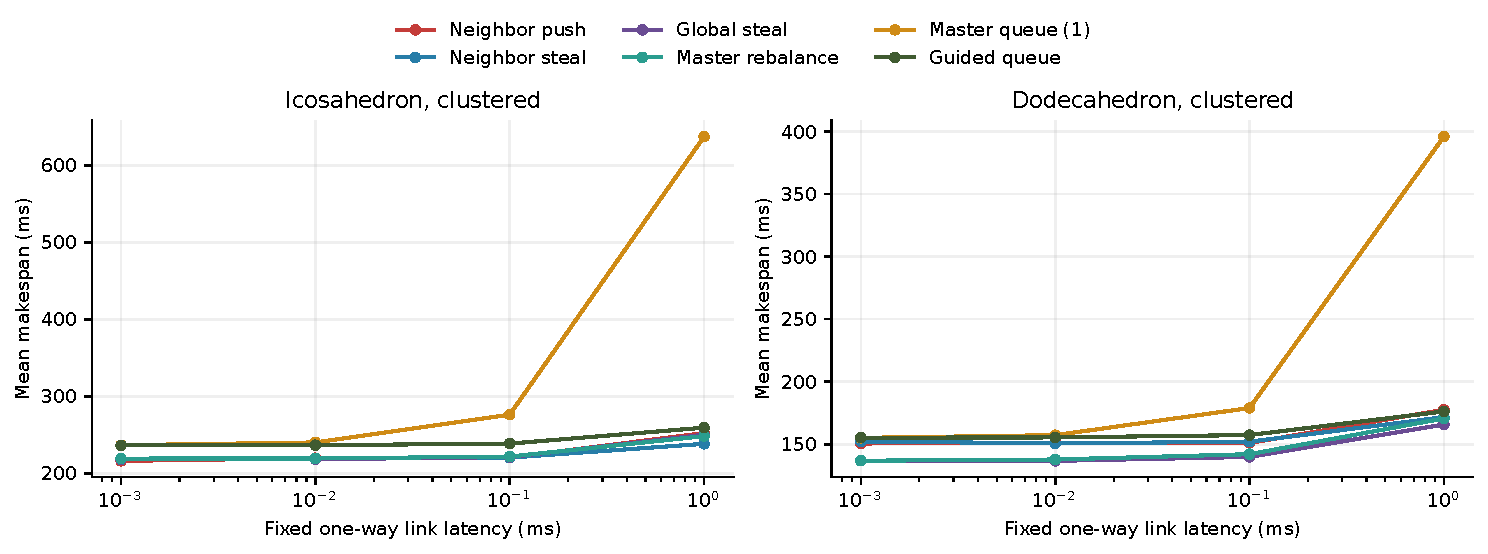
\includegraphics[width=.90\textwidth]{latency.pdf}
\caption{Clustered workload with identical fifteen-seed subsets. Bandwidth remains 100 MiB/s. Increasing fixed latency particularly penalizes single-task central requests; all points still use stable links.}
\label{fig:latency}
\end{figure*}

\begin{figure*}[!t]
\centering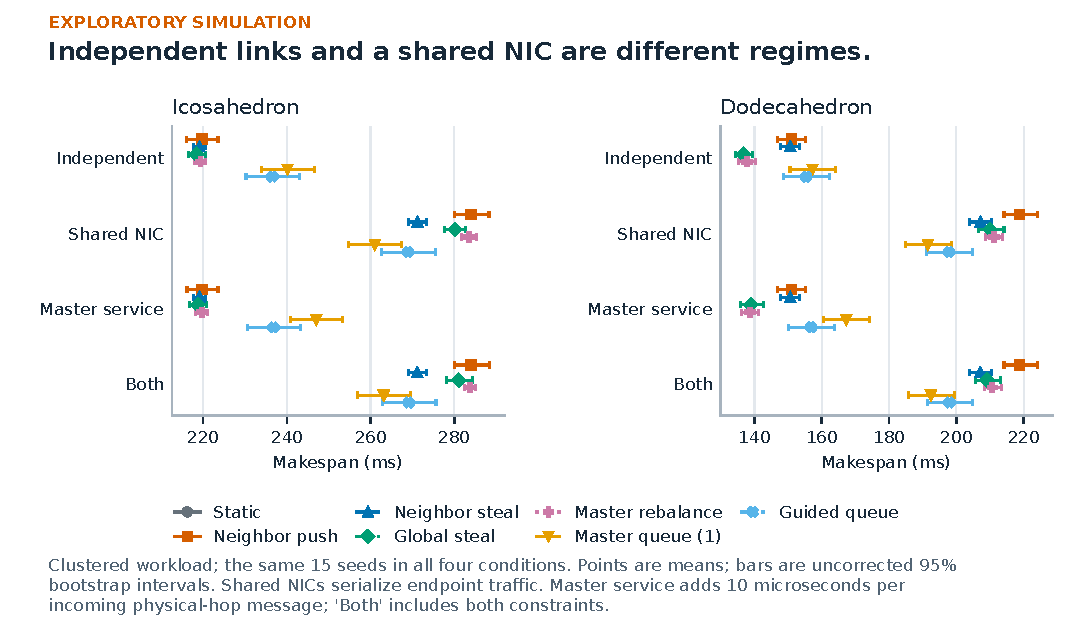
\includegraphics[width=.90\textwidth]{bottlenecks.pdf}
\caption{Shared endpoint serializers and serialized master service, clustered workload, fifteen paired seeds. Independent links are the primary baseline; a shared NIC changes startup concurrency and subsequent contention. The combined sensitivity uses both restrictions.}
\label{fig:bottlenecks}
\end{figure*}

At 1-ms link latency, dodecahedral clustered push takes 177.57 ms, local stealing 171.61 ms, master rebalancing 170.62 ms, and single-task master scheduling 395.85 ms. Guided batching takes 176.23 ms. At only 10 MiB/s, push takes 212.70 ms while guided scheduling takes 198.14 ms. Larger bulk migrations incur enough communication cost to change the ranking.

With shared NICs, dodecahedral clustered push takes 218.73 ms, local stealing 207.10 ms, and single-task master scheduling 191.56 ms. These are the same fifteen seeds, not the thirty-seed primary means. The primary model's simultaneous spoke transfers require independent aggregate link capacity; a shared master transmitter serializes the initial chunks. Smaller central requests can overlap distribution and computation, which changes the tradeoff. Adding a 10-$\mu$s master processing requirement alone has a smaller effect at these settings.

Donation and retry sensitivities are included in the companion summary CSV. For example, changing the dodecahedral clustered donation fraction to 3/4 gives push 141.65 ms; an eight-task cap gives 145.73 ms. Those observations are parameter explorations, not a tuned-policy claim tested on independent holdout workloads. Both 120-task and 9600-task cases complete correctly; they preserve 1-ms mean task cost, so total work changes deliberately in that sensitivity.

\subsection{Does Platonic Connectivity Add a Benefit?}
\begin{figure*}[!t]
\centering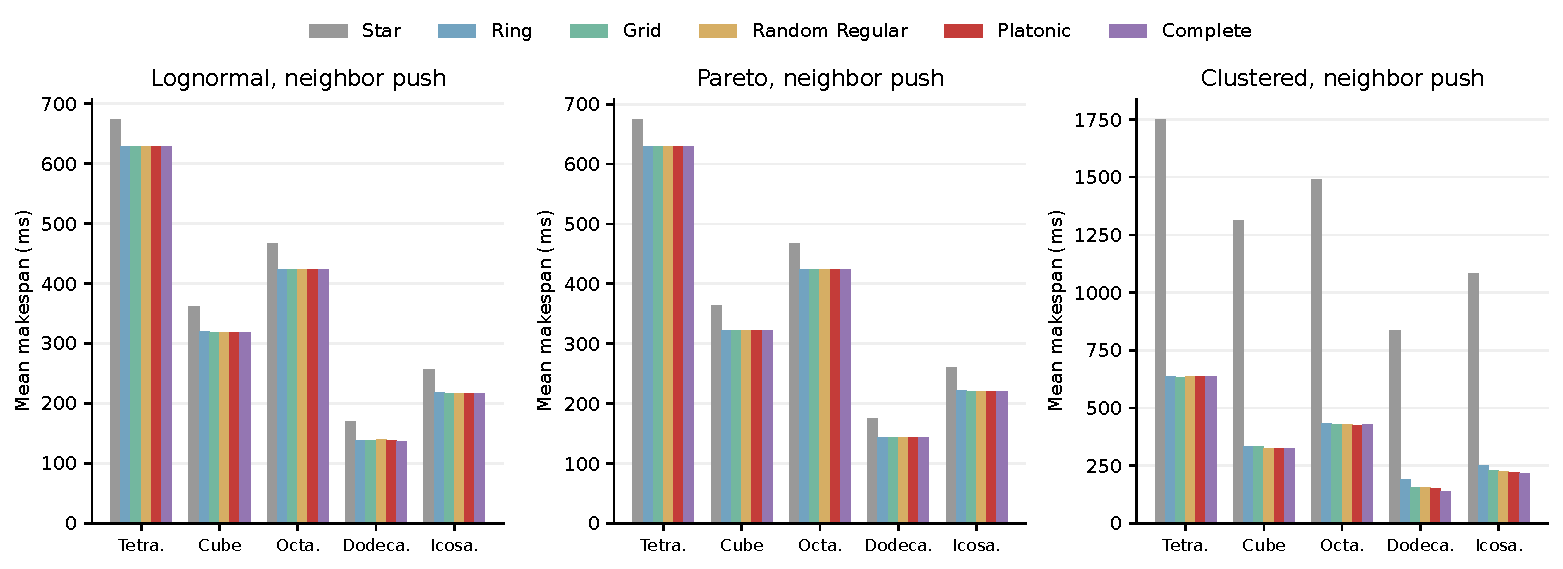
\includegraphics[width=.95\textwidth]{topologies.pdf}
\caption{Peer-topology controls using the same neighbor-push protocol, master spokes, worker count, and task instances within each solid size. Rewired controls match peer degree and link count; the other alternatives have different physical peer-link budgets. Thirty seeds per cell.}
\label{fig:topologies}
\end{figure*}

The topology experiment distinguishes access to peers from a unique geometric advantage. Rings and grids often make redistribution more constrained; complete connectivity provides a capacity reference. Neither comparison holds wiring cost constant. The degree-preserving control is therefore the more relevant comparison for claims about the special arrangement of Platonic edges.

For dodecahedral clustered push, the mean paired ratio $T_{\rm Platonic}/T_{\rm rewired}$ is 0.970 [0.946, 0.994], a modest exploratory advantage for the Platonic graph in that stress case. For dodecahedral independent lognormal costs it is 0.995 [0.984, 1.007], which does not establish an advantage. Icosahedral clustered work gives 0.984 [0.966, 1.002], also including equality. Conversely, icosahedral Pareto work gives 1.004 [1.000, 1.007], a small effect in the other direction. Full-precision values are provided in the topology summary. These uncorrected intervals and the selected rewiring procedure do not support general geometric superiority.

Because all physical links have identical speed and latency, the simulator does not assign performance value to three-dimensional placement itself. It measures the adjacency graph's opportunities and communication paths. Geometry may have practical packaging or wiring implications, but those would require a distance- or hardware-aware study beyond the requested stable-link assumptions.

\section{Limitations and Reproducibility}
The model omits failures, recovery, result reduction, cache behavior, memory limits, operating-system scheduling, task dependencies, worker-side control CPU overhead, and fluctuating capacity. Queued inputs must be copied on every migration. Tasks cannot be divided after execution begins. A single very expensive running task can dominate the makespan even if every other worker is idle. The stable-link assumption prevents modeling congestion-induced bandwidth reduction; queue serialization and the NIC variant account for the explicitly selected resource contention only.

The clustered workload is intentionally favorable to redistribution relative to static allocation. Other real workloads may already be shuffled or deliberately cost-balanced. We do not implement clairvoyant longest-processing-time scheduling because task costs are unknown in this model. Literature-inspired policies are finite-network implementations with documented batching and retry choices; they are not a performance evaluation of real work-stealing runtimes.

Thirty seeds provide uncertainty over the chosen synthetic distributions; they do not cover every task family or network setting. Multiple comparisons and parameter exploration call for restrained interpretation. A physical experiment could test measured task distributions, transport overheads, shared endpoint capacity, and master processing costs. Deployment claims require those measurements.

The study package includes simulator source, 116 tests, raw run CSV files, bootstrap summaries, full-precision paired effects, topology results, all PDF/PNG plots, and this LaTeX source. Python 3.12.14, NumPy 2.3.5, SciPy 1.17.0, Matplotlib 3.10.8, and pytest 8.4.2 were used. The bundled unmodified IEEEtran 1.8a class enables the requested two-column journal layout; its source commit and checksum are documented. The study README lists commands to rerun measurements, regenerate figures, and compile the paper. Raw timings are simulated milliseconds and are independent of the execution machine's CPU speed.

\section{Conclusion}
Neighbor work sharing on master-centered Platonic networks consistently reduces static-partition imbalance for the variable-cost workloads tested. Under independent 100-MiB/s links and 10-$\mu$s latency, the mean paired improvement over static is 1.074--1.228 for independent lognormal costs and 2.763--5.630 for the clustered stress case. Equal-cost workloads provide no redistribution benefit. Local stealing, global stealing, master rebalancing, and guided scheduling often match or improve on push, and communication assumptions can reverse rankings. Degree-matched controls establish no general advantage of Platonic connectivity. The defensible outcome is a reproducible, qualified assessment of a useful neighbor-sharing policy, rather than a universal claim about the best solid or best scheduler.

\begin{thebibliography}{5}
\bibitem{eager} D. L. Eager, E. D. Lazowska, and J. Zahorjan, ``Adaptive load sharing in homogeneous distributed systems,'' \emph{IEEE Trans. Softw. Eng.}, vol. SE-12, no. 5, pp. 662--675, 1986.
\bibitem{blumofe} R. D. Blumofe and C. E. Leiserson, ``Scheduling multithreaded computations by work stealing,'' \emph{J. ACM}, vol. 46, no. 5, pp. 720--748, 1999, doi: 10.1145/324133.324234.
\bibitem{guided} C. D. Polychronopoulos and D. J. Kuck, ``Guided self-scheduling: A practical scheduling scheme for parallel supercomputers,'' \emph{IEEE Trans. Comput.}, vol. C-36, no. 12, pp. 1425--1439, 1987.
\bibitem{graham} R. L. Graham, ``Bounds on multiprocessing timing anomalies,'' \emph{SIAM J. Appl. Math.}, vol. 17, no. 2, pp. 416--429, 1969.
\bibitem{coxeter} H. S. M. Coxeter, \emph{Regular Polytopes}, 3rd ed. New York, NY, USA: Dover, 1973.
\end{thebibliography}
\end{document}
